\documentclass[a4paper]{report}

%====================== PACKAGES ======================

\usepackage[french]{babel}
\usepackage[utf8]{inputenc}
%pour gérer les positionnement d'images
\usepackage{float}
\usepackage{amsmath}
\usepackage{graphicx}
%pour les informations sur un document compilé en PDF et les liens externes / internes
\usepackage{hyperref}
%pour la mise en page des tableaux
\usepackage{array}
\usepackage{tabularx}
%pour utiliser \floatbarrier
%\usepackage{placeins}
%\usepackage{floatrow}
%espacement entre les lignes
%modifier la mise en page de l'abstract
%police et mise en page (marges) du document
\usepackage[T1]{fontenc}
\usepackage[top=2cm, bottom=2cm, left=2cm, right=2cm]{geometry}
%Pour les galerie d'images

\usepackage{multicol}
\usepackage{float}

%====================== INFORMATION ET REGLES ======================

%rajouter les numérotation pour les \paragraphe et \subparagraphe
\setcounter{secnumdepth}{5}
\setcounter{tocdepth}{5}



%======================== DEBUT DU DOCUMENT ========================

\begin{document}

%régler l'espacement entre les lignes
\newcommand{\HRule}{\rule{\linewidth}{0.5mm}}

%page de garde
\begin{titlepage}
\begin{center}

% Upper part of the page. The '~' is needed because only works if a paragraph has started.

\includegraphics[width=\textwidth]{./logo}~\\[1cm]

%\textsc{\LARGE Université ou Entreprise}\\[1.5cm]

\textsc{\Large }\\[0.5cm]

% Title
\HRule \\[0.4cm]

{\huge \bfseries Rapport ST4:\\
[0.4cm] }

{\large \bfseries EI Mondor\\[0.4cm] }

{\large \bfseries \textit{Détection du type de cancer du foie et prédiction de la survie}\\[0.4cm] }


\HRule \\[1.5cm]

\vspace{3cm}

% Author and supervisor
\begin{minipage}{0.4\textwidth}
\begin{flushleft} \large
\emph{Réalisé par le groupe:}\\
	Marilou \textsc{Bernard de Courville}\\
	Amram \textsc{El Bazis}\\
	Reda \textsc{Hamama}\\
	Alexis \textsc{Le Parco}\\
	Adiel \textsc{Van Hecke}\\
\end{flushleft}

\end{minipage}


\vfill

% Bottom of the page
{\large \today}

\end{center}
\end{titlepage}



%\tableofcontents
%\thispagestyle{empty}
%\setcounter{page}{0}
%ne pas numéroter le sommaire

%\newpage

%espacement entre les lignes d'un tableau
\renewcommand{\arraystretch}{1.5}

%====================== INCLUSION DES PARTIES ======================

\begin{multicols}{2}
~
\thispagestyle{empty}
%recommencer la numérotation des pages à "1"
\setcounter{page}{0}
\newpage

\chapter{Introduction}
\label{ch:Introduction}

Dans le cadre de notre ST4 \textit{Big Data et Santé}, nous avons choisi l'enseignement d'intégration en partenariat avec le service de radiologie de l'hôpital Henri Mondor. Notre projet consiste à développer un outil d'aide à la décision pour la détection du type de cancer du foie et la prédiction de la survie des patients.

\section{Données}

Notre approche repose donc sur des données anonymisées fournies par l'hôpital Henri Mondor, qui comprennent des données radiomiques, cliniques, et d'observations médicales. Ces données sont réparties dans plusieurs tableaux. Les patients sont identifiés par le couple \texttt{(patient\_num, classe\_name)}, où \texttt{patient\_num} est le numéro du patient et \texttt{classe\_name} est le type de cancer du foie. Les types de cancer du foie présents dans le dataset sont les suivants: CCK, CHC et Mixtes. De plus, on prend en compte différentes phases d'injections, dans \texttt{temps\_inj}, qui sont: artérielle, portale et veineuse et tardive, notées respectivement \texttt{ART, PORT, VEIN, TARD}. De plus, nous avons un set de données contenant des coupes de la tumeur, nous donnant des informations sur la taille et l'intérieur de la tumeur.

Voici donc des statistiques sur le dataset que nous avons utilisé:

\begin{figure}[H]
\centering
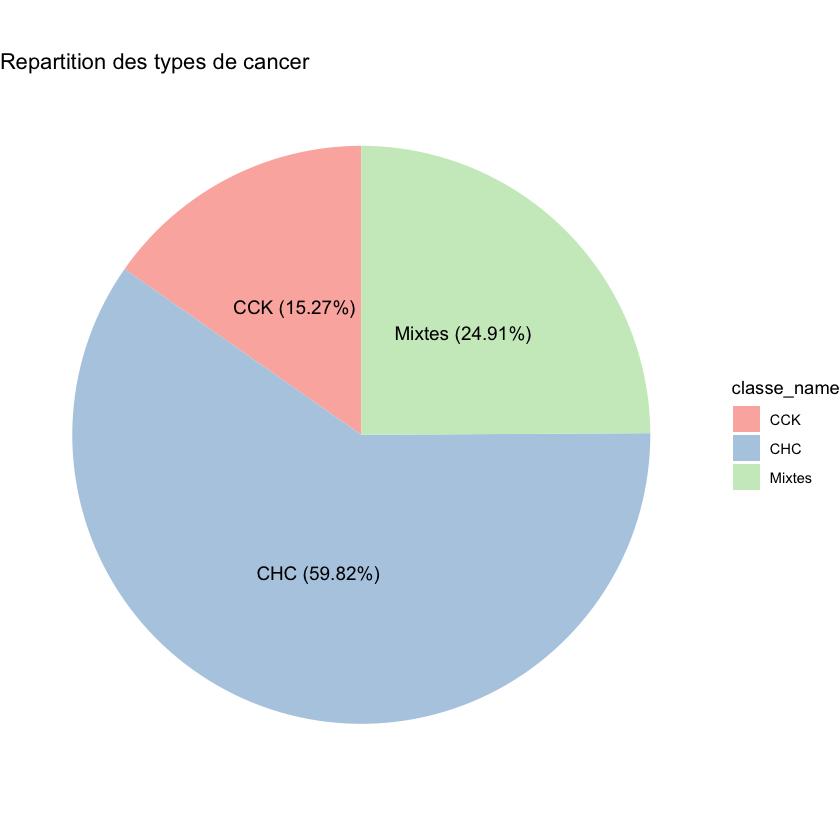
\includegraphics[width=0.23\textwidth]{img/repartition-type.png}
\caption{Répartition des types de cancer du foie dans le dataset}
\end{figure}

\begin{figure}[H]
\centering
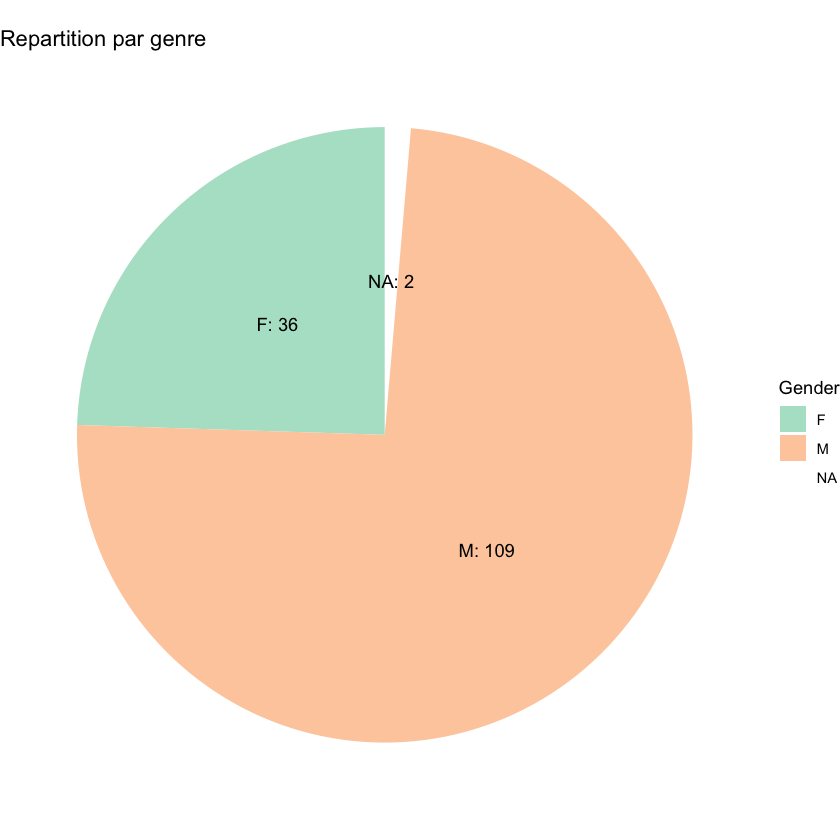
\includegraphics[width=0.23\textwidth]{img/repartition-genre.png}
\caption{Répartition des genres dans le dataset}
\end{figure}

\begin{figure}[H]
\centering
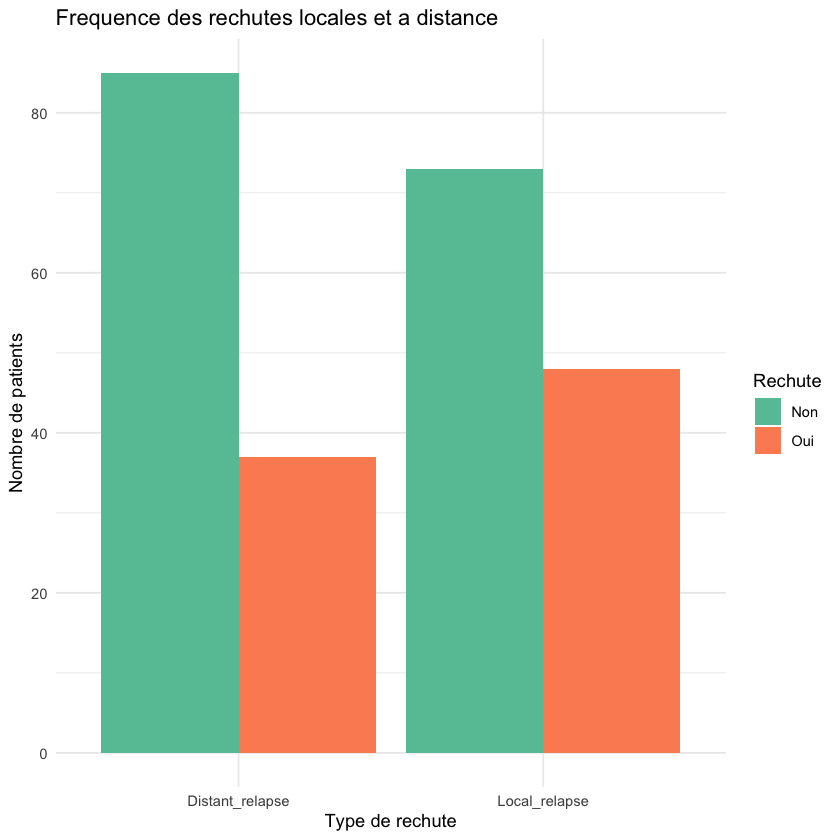
\includegraphics[width=0.23\textwidth]{img/freq-rechute.png}
\caption{Fréquence de rechute des patients, par type de rechute}
\end{figure}

\begin{figure}[H]
\centering
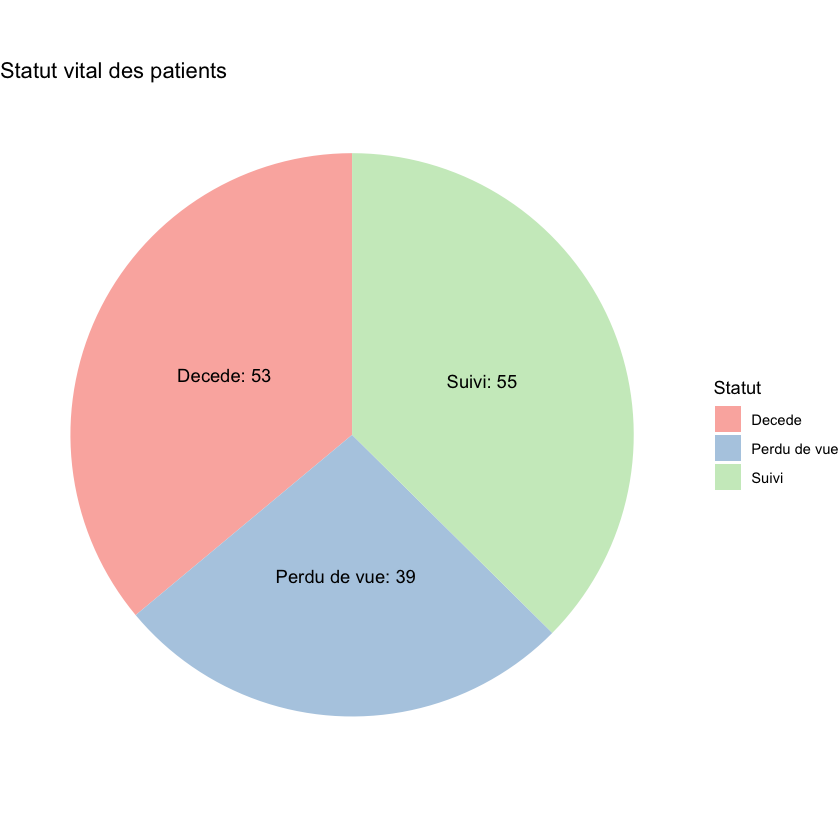
\includegraphics[width=0.23\textwidth]{img/statut-vital.png}
\caption{Statut vital des patients}
\end{figure}

\begin{figure}[H]
\centering
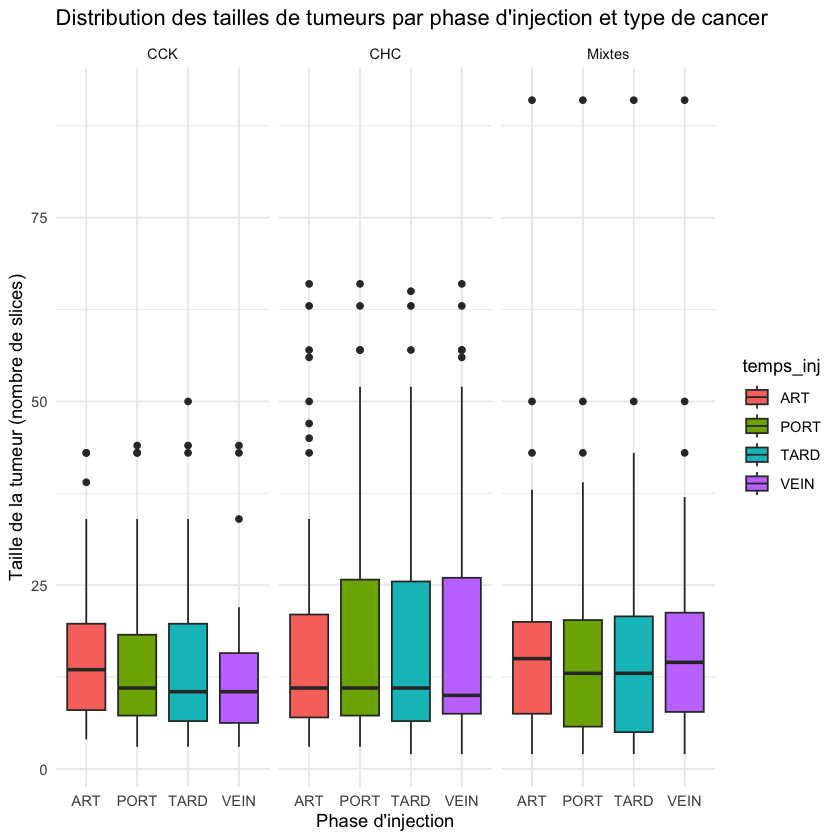
\includegraphics[width=0.23\textwidth]{img/taille-cancer.png}
\caption{Distribution de la taille des cancers par type de cancer et par phase}
\end{figure}

En tout, nous avons un dataset de 148 patients.

On remarque que le dataset est déséquilibré, contenant une majorité de patients atteints de CHC, et une minorité de patients atteints de CCK. De plus, on remarque que la majorité des patients sont des hommes.


\chapter{Démarches}
\label{ch:modele_continu}

\section{Traitement des données}
\subsection{Contexte}
Plusieurs dataset ont été utilisés pour cette étude, des données sur le descriptif des patients, sur les résultats radiomiques globaux
et multislice des patients sur leur tumeur, et enfin un jeu de données sur les observations visuelles des radiologues.
Beaucoup de données non analysables ont été retirés des dataset pour ne garder que les informations sur la forme, le niveau de gris et les textures.

\subsection{Multislicing}

L'avantage du jeu de données multislice est d'avoir des métriques sur chaque coupe de la tumeur. 
Ceci dit, la difficulté derrière est qu'un numéro de slice ne défnisse pas une région fixe du foie entre les patients
ni entre les phases d'un même patient.\\
Aussi faut-il traiter les données pour les rendre exploitables et comparables entre les patients. 
Pour ce faire, la démarche suivie est de déterminer des nouvelles métriques sur les courbes des variables en fonction
des slices (Voir Figure 2.1.)
\begin{figure}[H]
    \centering
    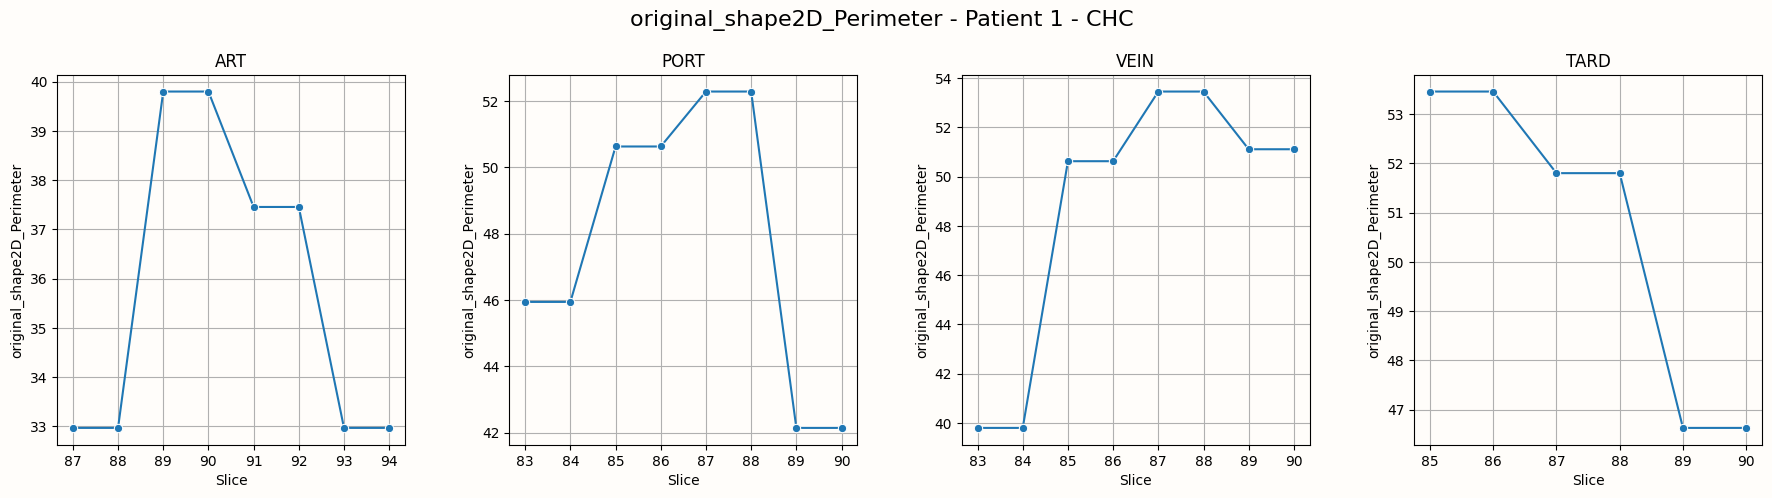
\includegraphics[width=0.5\textwidth]{img/perimeter.png}
    \caption{Courbe représentant le périmètre en fonction des slices sur les différentes phases d'un patient}
    \label{fig:perimeter}
\end{figure}

Plusieurs variables, décrivant les variations locales, ont été extraites notamment la moyenne, l'écart-type, 
la symétrie et l'énergie.

\subsection{Sélection des variables}
Une fois les données traitées, nous avons utilisé une analyse des composantes principales pour sélectionner les variables les plus 
informatives. 

\chapter{Résultats}
\label{ch:ch3}

Durant cet enseignement d'intégration, nous avons obtenu de nombreux résultats, en particulier en combinant différents jeux de données (global, multislice et visuel).
Dans cette partie, nous nous concentrerons sur les deux résultats principaux.

\section{Modèles}

Dans un premier temps, notre travail s'est focalisé sur deux modèles de classification : la forêt aléatoire \textit{Random Forest} et la régression logistique.

\vspace{0.3cm}

Pour assurer le bon fonctionnement de nos programmes, ces modèles s'appuient sur deux fonctions essentielles : \texttt{SMOTE} et \texttt{GroupShuffleSplit}.

\vspace{0.3cm}

\texttt{SMOTE} permet de rééquilibrer les classes dans le jeu d'entraînement.

\texttt{GroupShuffleSplit} garantit que les différentes phases d'un même patient ne soient pas séparées entre le jeu d'entraînement et le jeu de test.

\section{Résultat 1 : AUC pour le dataset global}

\begin{figure}[H]
\centering
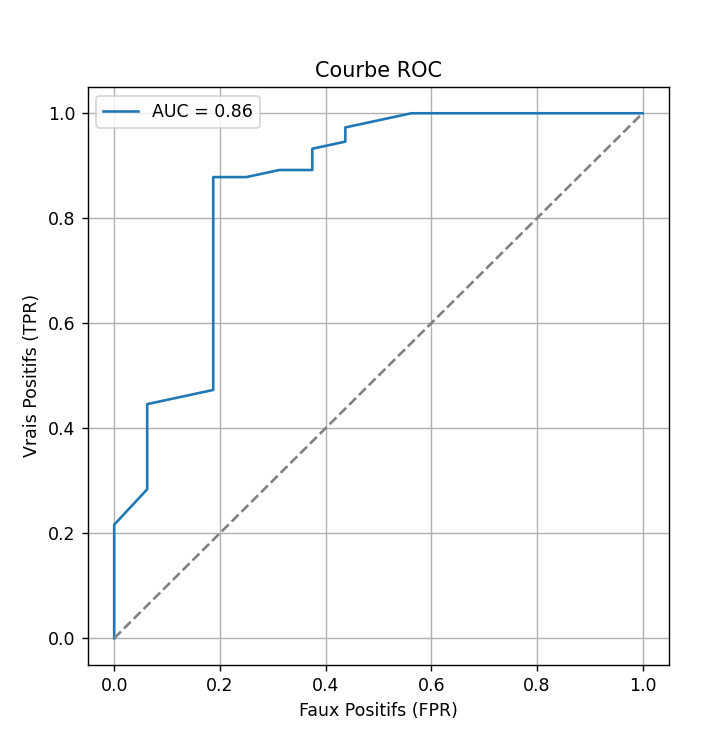
\includegraphics[width=0.3\textwidth]{img/AUC_global.png}
\caption{AUC pour le dataset global}
\label{fig:auc_global}
\end{figure}

\vspace{0.5cm}

On observe une valeur d'AUC de 0{,}84, ce qui correspond à un modèle globalement performant.
\chapter{Régression Lasso}
\label{ch:ch4}
La méthode précédente produisant des variables d’importance relativement homogène, elle rend l’interprétation difficile. Afin de permettre aux radiologues d’identifier plus facilement les variables pertinentes ainsi que leur mode d’influence, nous avons exploré une approche alternative plus interprétable.

Nous avons ainsi réalisé une régression logistique en utilisant l’ensemble de nos paramètres numériques, identifiés par leur phase d'injection, comme variables explicatives, et la variable \texttt{Classe\_name} (valant 1 pour CHC et 0 pour CKC) comme variable cible. Pour l'entraînement du modèle, nous avons utilisé 80\,\% des données disponibles.

Les données de train et de test sont créées avec de l’échantillonnage stratifié pour avoir la même proportion de classe dans les deux ensembles,

La régression aboutit à une équation de la forme :
\[
\scriptstyle
Y = \beta X,\quad \text{avec } \beta = (\beta_1, \dots, \beta_{528}), \; X = (X_1, \dots, X_{528}),
\]
où les coefficients $\beta_j$ sont estimés par maximisation de la vraisemblance.

Afin de sélectionner uniquement les variables les plus pertinentes, nous avons appliqué une pénalisation de type \textit{Lasso} (L1). Cette méthode force certains coefficients $\beta_j$ à s’annuler, ne conservant que ceux dont l’impact est significatif sur la prédiction. Cela permet une meilleure interprétation du rôle de chaque variable dans la classification.

Nous avons ensuite tracé la courbe ROC du modèle (représentant le taux de vrais positifs en fonction du taux de faux positifs pour chaque seuil de classification). Le point optimal, situé le plus près du coin supérieur gauche du graphique, correspond à un seuil de classification de 0{,}21. À ce seuil, le modèle atteint une précision de 80\,\%, mais la sensibilité (c’est-à-dire la capacité du modèle à détecter correctement les cas positifs, ici les CKC) n’est que de 57\,\%.

\begin{figure}[H]
    \centering
    \includegraphics[width=0.4\textwidth]{img/roc.jpg}
    \caption{Figure: Courbe ROC}
\end{figure}


Cette faible sensibilité s’explique en grande partie par le déséquilibre entre les classes. C’est pourquoi nous nous intéressons également à la précision pondérée, qui atteint 72\,\% et prend en compte le déséquilibre des classes dans l’évaluation globale du modèle.

Une analyse du modèle donne comme variables prépondérantes les variables : 

\begin{table}[H]
    \centering
    \resizebox{\columnwidth}{!}{
    
    \begin{tabular}{|c|c|c|}
    \hline
    \textbf{Niveau de gris} & \textbf{Forme} & \textbf{Texture} \\
    \hline
    \texttt{original\_firstorder\_10Percentile} & \texttt{original\_shape\_Elongation} & \texttt{original\_gldm\_DependenceVariance}, \\
     & & \texttt{DependenceEntropy}, \\
     & & \texttt{LargeDependenceHighGrayLevelEmphasis} \\
    \hline
    \texttt{original\_firstorder\_Energy} & \texttt{original\_shape\_Sphericity} & \texttt{original\_glcm\_InverseVariance} \\
    \hline
    \texttt{original\_firstorder\_Skewness} & & \texttt{original\_glszm\_GrayNonUniformityNormalized}, \\
    & & \texttt{SmallAreaLowGrayLevelEmphasis} \\
    \hline
    \texttt{original\_firstorder\_TotalEnergy} & & \\
    \hline
    \end{tabular}}
    \caption{Tableau des variables radiomiques sélectionnées}
    \end{table}
Les variables les plus influentes sont celles avec un coefficient absolu le plus élevé, les négatives indiquant une augmentation de la probabilité d’être classé comme CKC et les positives d'être CHC.La distriubtion des coefficients est représentée dans la figure suivante.
\begin{figure}[H]
    \centering
    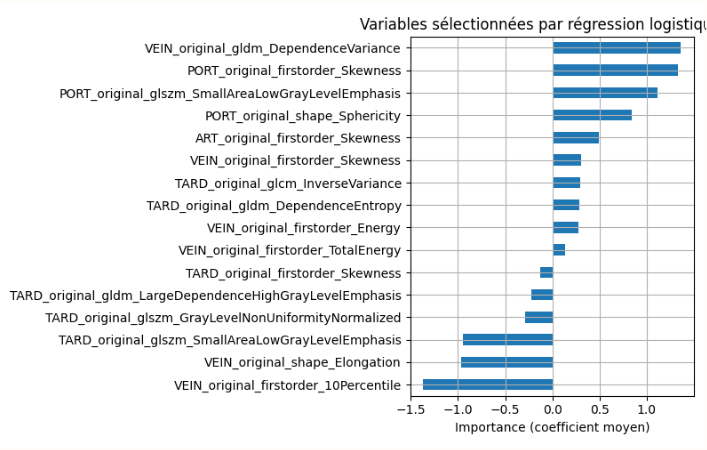
\includegraphics[width=0.5\textwidth]{img/variables.png}
    \caption{Influence des variables sélectionnées}
\end{figure}

\input{Chapitre5.tex}

\chapter{Conclusion}
\label{ch:Conclusion} 


En conclusion, au cours de notre projet, nous avons pu établir deux types de modèles complémentaires permettant de déterminer le type de cancer du foie. 
Par ailleurs, l’utilisation du score dans l’analyse de survie nous a permis d’identifier des variables pertinentes associées à la survie des patients. 

En perspective, il serait pertinent d’exploiter une base de données plus équilibrée en termes de répartition des classes afin de construire un modèle de classification dédié à l’analyse de survie.
De plus, il est intéressant de noter que l'on aurait pu étudier la durée de la survie des patient, alors que l'on a simplement étudier binairement si un patient survivait ou non.



\end{multicols}

\end{document}